% !TEX root=../../thesis.tex
\clearpage
\section{Case study of similiar systems}
\label{sect:backgroundExamples}
This section will present some similar systems and we will explain what the
systems try to present.
\subsection{Zugmonitor}
\label{sub:subsection_zugmonitor}

In the Zugmonitor (see \vref{fig:zugmonitor}) each long-distance 
trains in the German railway network has been plotted as a arrow on a German 
map. To illustrate the punctuality of each train, a colored circle has been 
added to each arrow if the train is delayed with varying color depending on 
how big the delay is. A time line is also displayed to see how the trains run 
on each step of the routes. 

\begin{figure}[!htbp]
	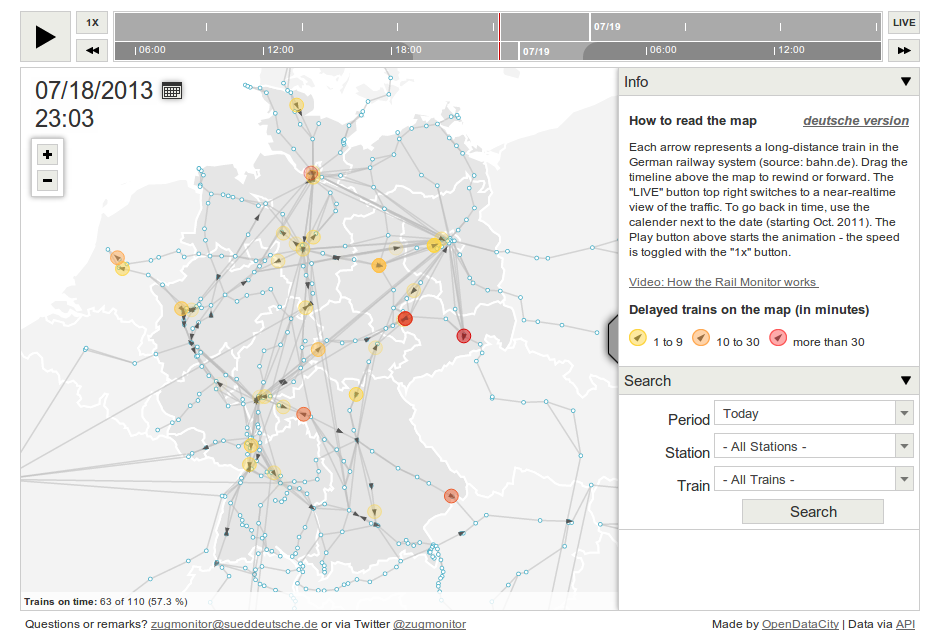
\includegraphics[width=\textwidth,center]{zugmonitor.png}
	\caption[Zugmonitor]{Zugmonitor \cite{zugmonitor}}
	\label{fig:zugmonitor}
\end{figure}
\pagebreak

\clearpage
\subsection{Vaguely live map of trains in the United Kingdom}
\label{sub:subsection_ukLiveMap}

This is a map which plots the relative location of each train in the United
Kingdom (see \vref{fig:ukLiveMap}). The plot fetches the departure time from the 
National Rail website and calculates the relative location. The plot does not
indicate whether the trains are on schedule or delayed, this must be
done either manually, or for instance by checking a time table\cite{trainTimesUK}.
Both the map and time table is developed on hobby basis by the same person. 

\begin{figure}[!htbp]
	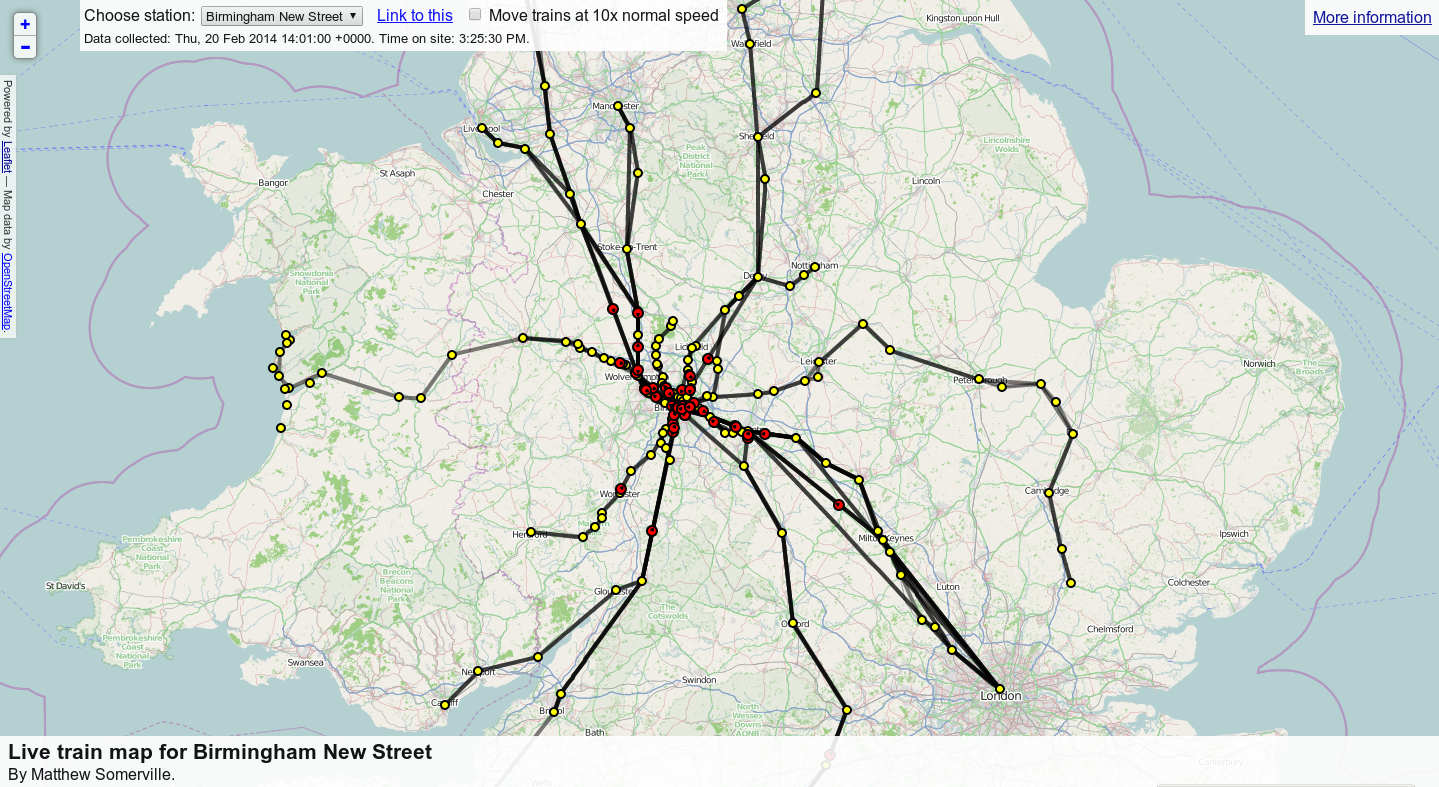
\includegraphics[width=\textwidth,center]{live-train-map-for-Birminingham-new-street.png}
	\caption[UK live map]{UK live map \cite{ukLiveMap}}
	\label{fig:ukLiveMap}
\end{figure}
\pagebreak

\clearpage
\subsection{MUNI Light Rail}
\label{sub:subsection_muniLightRail}

This a train graph based on the N-Judah line on the Muni Metro light railway line in San Francisco (see \vref{fig:muniLightRail}). 
This chart plots the schedule of the each train and the actual time each train 
uses. The chart auto updates every 10 seconds, and combined with being able 
to spot the difference between the schedule and the actual time, makes it easy 
to spot the delay of each train. As with \vref{sub:subsection_ukLiveMap} it 
has been developed on a hobby basis.

\begin{figure}[!htbp]
	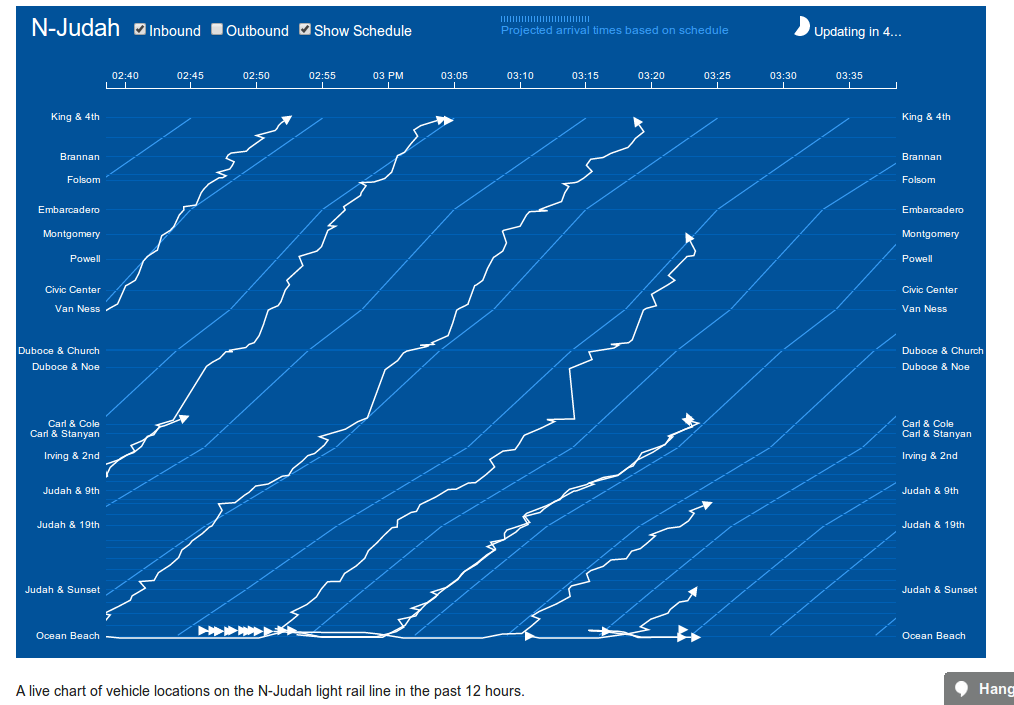
\includegraphics[width=\textwidth,center]{visualizing-transit-delays.png}
	\caption[MUNI Light Rail]{MUNI Light Rail \cite{muniLightRail}}
	\label{fig:muniLightRail}
\end{figure}
\pagebreak


\clearpage
\subsection{MiseryMap}
\label{sub:subsection_zugmonitor}

The MiseryMap (see \vref{fig:miserymap}) shows how much different airports and 
the routes between them are delayed. It also have a playback function to see 
the delays throughout the day. This plot also shows the weather sometimes so it
may be possible to spot if the delays is to be blamed on uncontrollable
conditions. 

\begin{figure}[!htbp]
	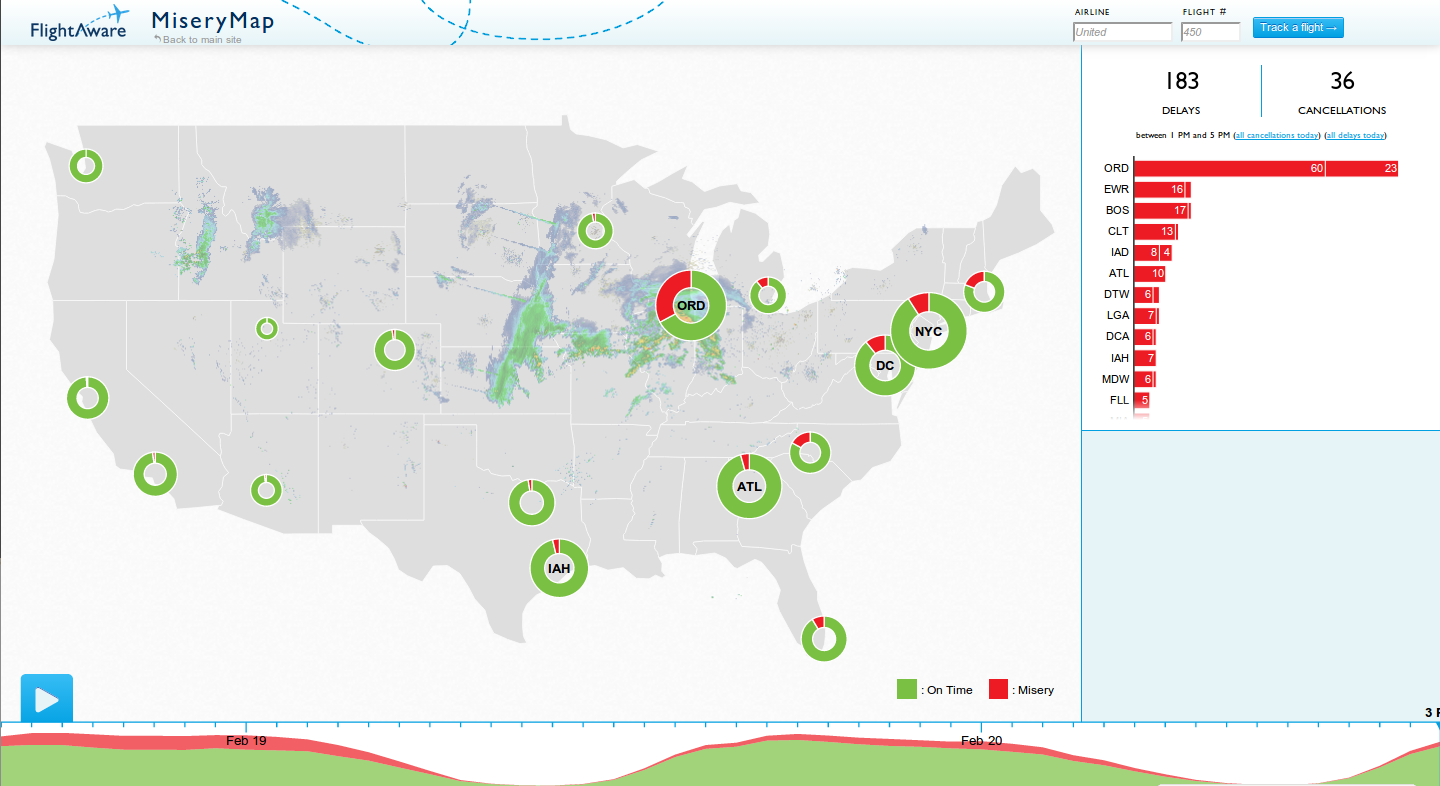
\includegraphics[width=\textwidth,center]{MiseryMap.png}
	\caption[MiseryMap]{MiseryMap \cite{flightAware:MiseryMap}}
	\label{fig:miserymap}
\end{figure}
%\pagebreak
 
\clearpage
\subsection{Norwegian National Rail Administration}
\label{sub:subsection_jernbaneverket}

Jernbaneverket is the Norwegian governments agency for railway services \cite{jernbaneverketAbout}.
This means that they are responsible for all the railway network in Norway.
Because of this, they also collect in data from points that each train passes, see \vref{fig:jernbaneverket-trafikkdata}. 
Based on this, they have recently released a map (see \vref{fig:jernbaneverket-punklighet}) over the punctuality on each stretch. This is a 
interactive map which shows a pop-up box containing the punctuality of the 
stretch clicked on, and this pop-up also shows which train routes that
operates this stretch. The map, does not however, show more information if 
the user zooms inn, which is possible within the map itself, and has a static 
view of Norway and the railway. This map only shows the punctuality for 
passenger trains, and not freight trains and/or both.\\ 

To analyze each stretch, on a detailed level between each station,
Jernbaneverket has a internal system called TIOS (see \ref{fig:jernbaneverket-tios}).
This is a train graph which plots all trains that passes between all stations,
in this example between Oslo S and Drammen, where the red lines means planned
time, black lines is actual time and the red circle indicates a a code for the cause of the delay. 

\begin{figure}[!htbp]
	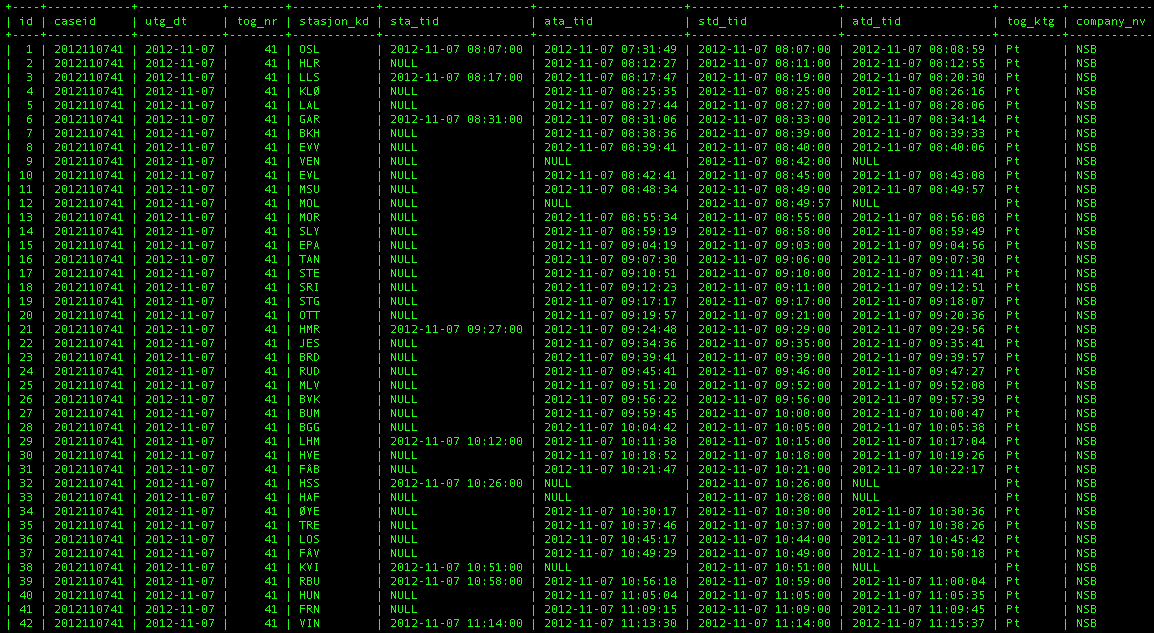
\includegraphics[width=\textwidth,center]{trafikkdata.png}
	\caption[Traffic data]{Traffic data	\cite{sintefPresis}}
	\label{fig:jernbaneverket-trafikkdata}
\end{figure}
\pagebreak

\begin{figure}[!htbp]
	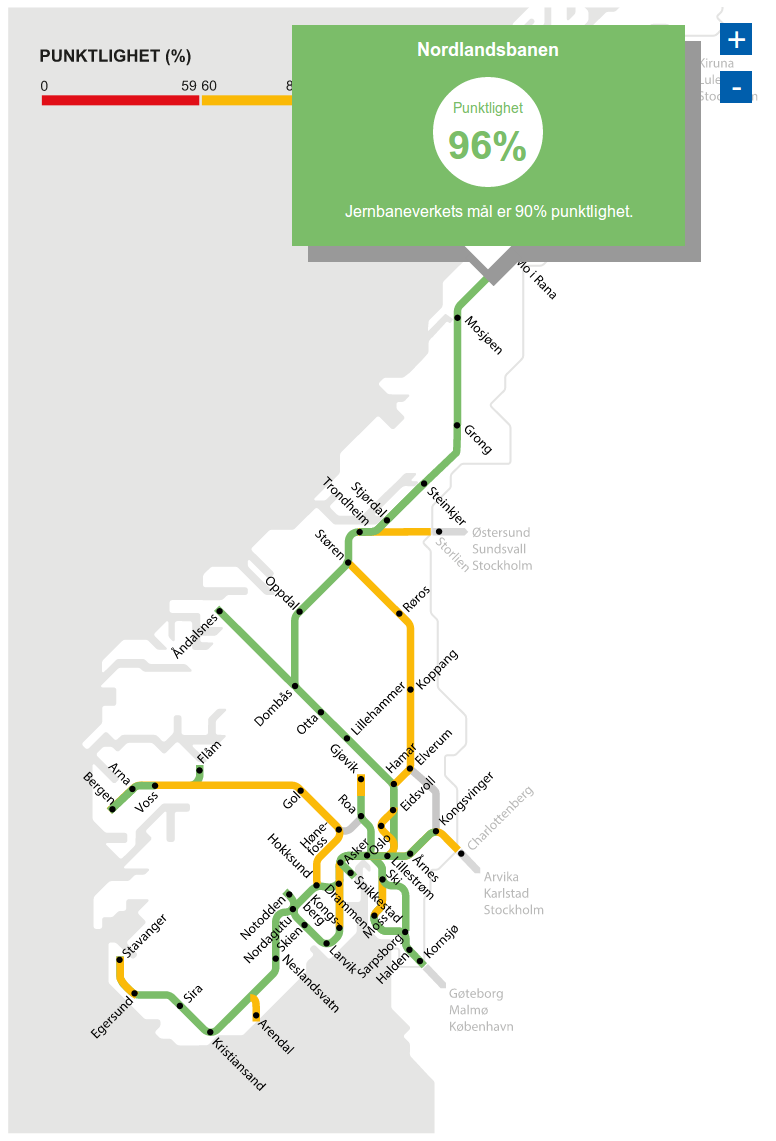
\includegraphics[height=\textheight,center]{jernbaneverket-punklighet.png}
	\caption[JBV Punctuality map]{JBV Punctuality map \cite{jernbaneverketPunklighetKart}}
	\label{fig:jernbaneverket-punklighet}
\end{figure}
\pagebreak

\begin{figure}[!htbp]
	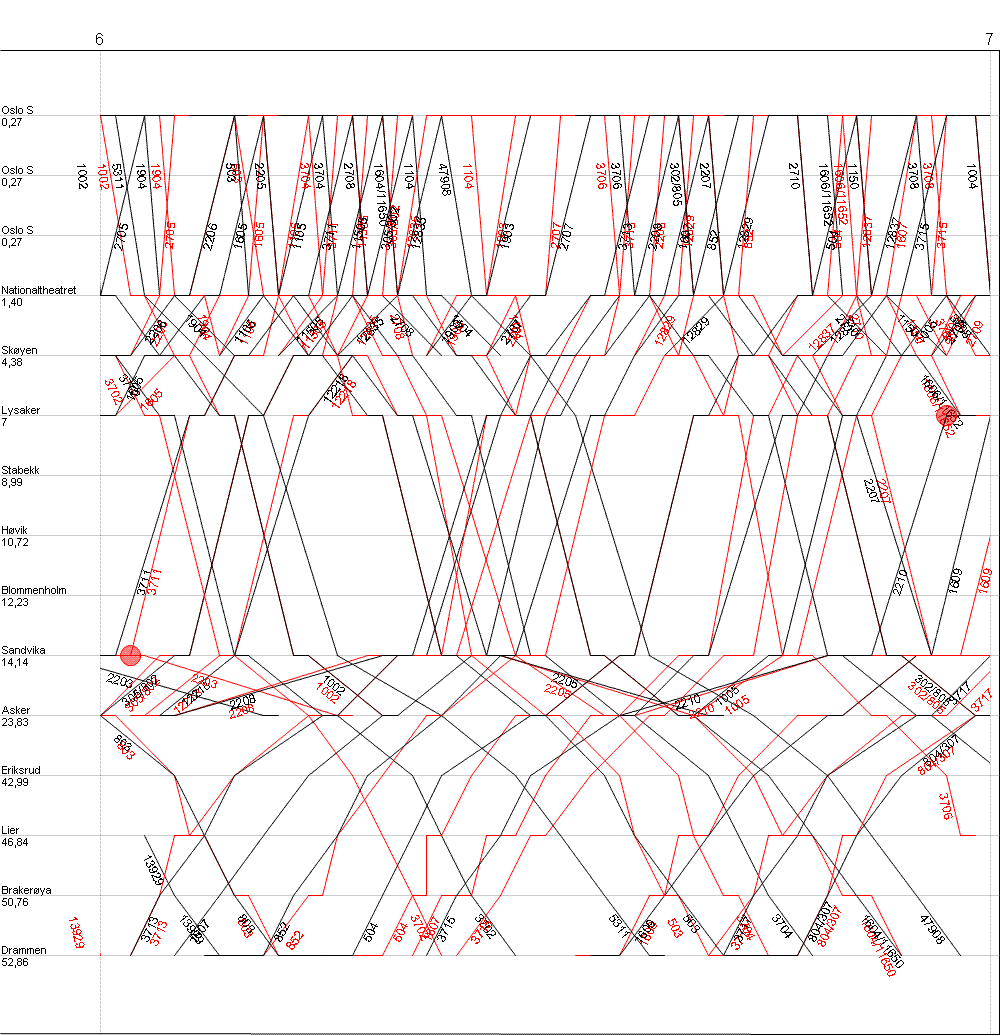
\includegraphics[width=\textwidth,center]{tios.png}
	\caption[TIOS]{TIOS\cite{jernbaneverketPunklighetKart}}
	\label{fig:jernbaneverket-tios}
\end{figure}
\pagebreak


\clearpage
\subsection{Tåg.info}
\label{sub:subsection_taag.info}

Tåg.info\cite{taagInfo} is a Swedish system that tracks SJ\cite{svenskaJernban} trains. The
service gathers and processes data from Trafikverket\cite{trafikverket}. As
with Cargonet (section \vref{sub:subsection_cargonet}), it provides a method (\vref{fig:taag-info-kart}) of
tracking live trains and visually see whether the trains are on schedule or
delayed. 

Tåg.info also provides a method of analyzing national delays by presenting
graphs, \vref{fig:taag-info-historik}. The service presents both a bar-chart
which presents the minutes of delays and the accumulated delays per day, and a
pie chart of the current status.

\begin{figure}[!htbp]
	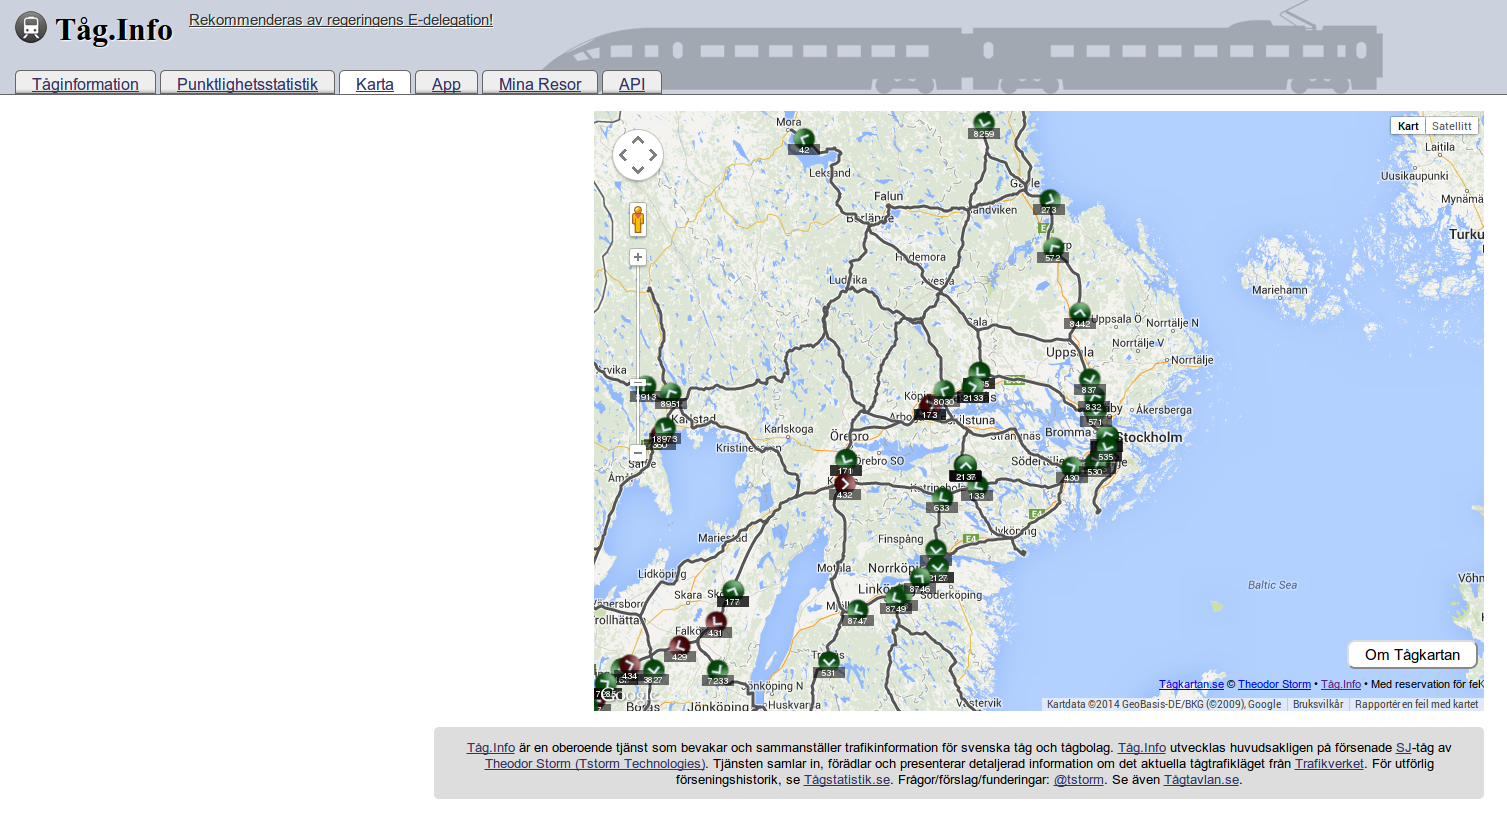
\includegraphics[width=\textwidth,center]{taag-info-kart.png}
	\caption[Tåg.info map]{Tåg.info map
	\cite{taagInfo}}
	\label{fig:taag-info-kart}
\end{figure}
\pagebreak

\begin{figure}[!htbp]
	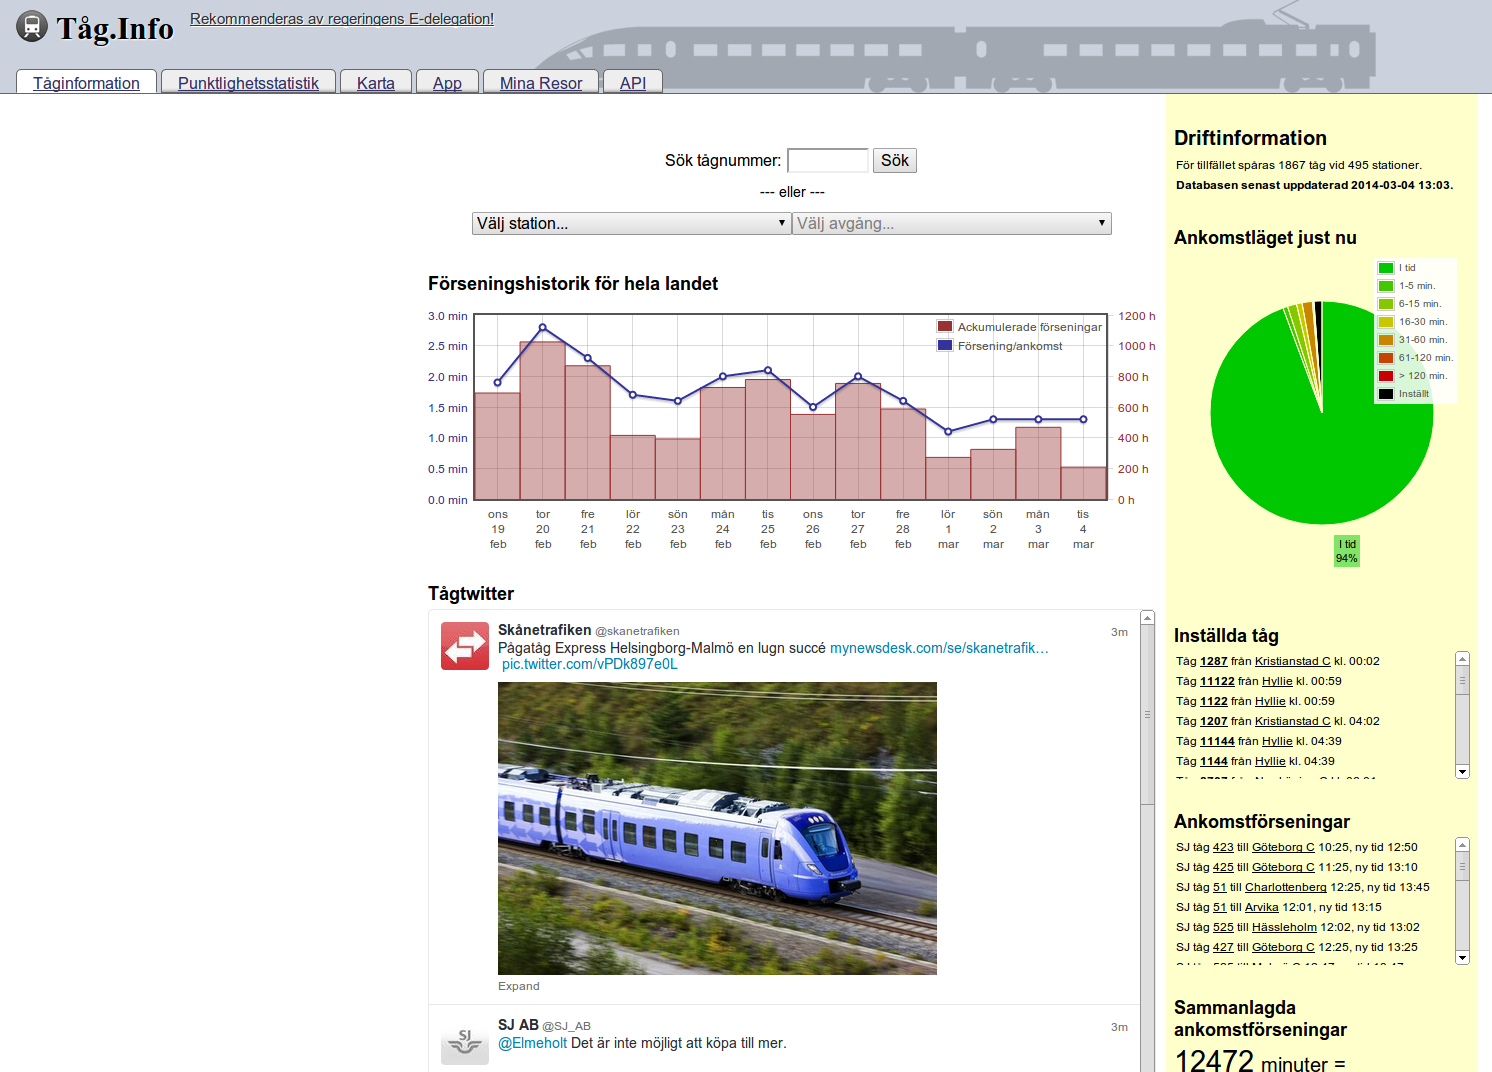
\includegraphics[width=\textwidth,center]{taag-info-historik.png}
	\caption[Tåg.info history]{Tåg.info history
	\cite{taagInfo}}
	\label{fig:taag-info-historik}
\end{figure}
\pagebreak


\clearpage
\subsection{SINTEF Presis}
\label{sub:subsection_sintefPresis}

The PRESIS\cite{sintefPresis} project is a project between SINTEF\cite{sintef},
Transportøkonomisk Institutt\cite{transportOkonomiskInstitutt},
NTNU\cite{ntnu}, Jernbaneverket(section \vref{sub:subsection_jernbaneverket}) 
and the train operators. The aim is to systematicly improve the precision 
level in the railway system by developing methods, tools, and processes. During
this project several prototypes for analyzing train delays have been developed.

A interaction plot, see \vref{fig:krysningsinteraksjon}, plots the interaction
between two selected trains at a selected station. This makes it easy to see 
if a train is delayed, and how it might affect another train. Since it only
plots between two trains, it makes it tedious to track large delays back 
throughout all interaction a train may have to find the source of the delay.
This makes it useful for individual trains, but makes it difficult to use if
one might look at the entire railway network or a large portion. \\

Publicly and internally it may differ if a train is delayed or not. Publicly
statistically data only shows delays on the final destination of the train, all
station along the route only shows there and then on information screens.
Since Jernbaneverket collects data from all signal points along the route (see \vref{fig:jernbaneverket-trafikkdata}), they
are able to track and plot the delays the train may experience along the route
and not only at the end station. The PRESIS project has develop a prototype for
such a plot, see \vref{fig:live-punklighet}. Here the circles represent a
station and the lines between the station have different 
colors which represent the punctuality between the stations, and the data which
it's based on are listed to the right. They have also made it possible to get a
time used over distance plot (see \vref{fig:plot-spc-for-strekning}) based on
the selected data in the Punctuality for routes plot. 

A plot based on time over distance, \ref{fig:plot-spc-for-strekning}, plots the
actual time used by all trains that have driven that stretch in the selected
time period along with the running average. This makes it possible where and
when trains have experienced problems on the selected stretch. They also have a
prototype plot which plots time used on station (see \vref{fig:plot-spc-for-stasjonsopphold})
and other prototypes which is similar, just focusing on other parts of the
process.  %Bidragsplot, ikke tatt med.



%\begin{figure}[!htbp]
%	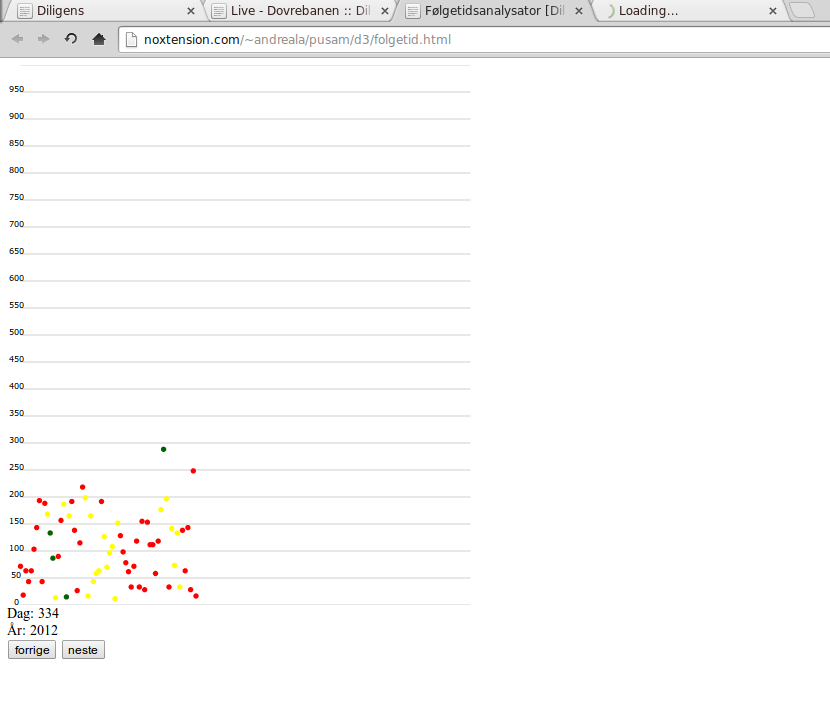
\includegraphics[width=\textwidth,center]{folgetid.png}
%	\caption[folgetid]{folgetid \cite{sintefPresis}}
%	\label{fig:folgetid}
%\end{figure}
%\pagebreak

%\begin{figure}[!htbp]
%	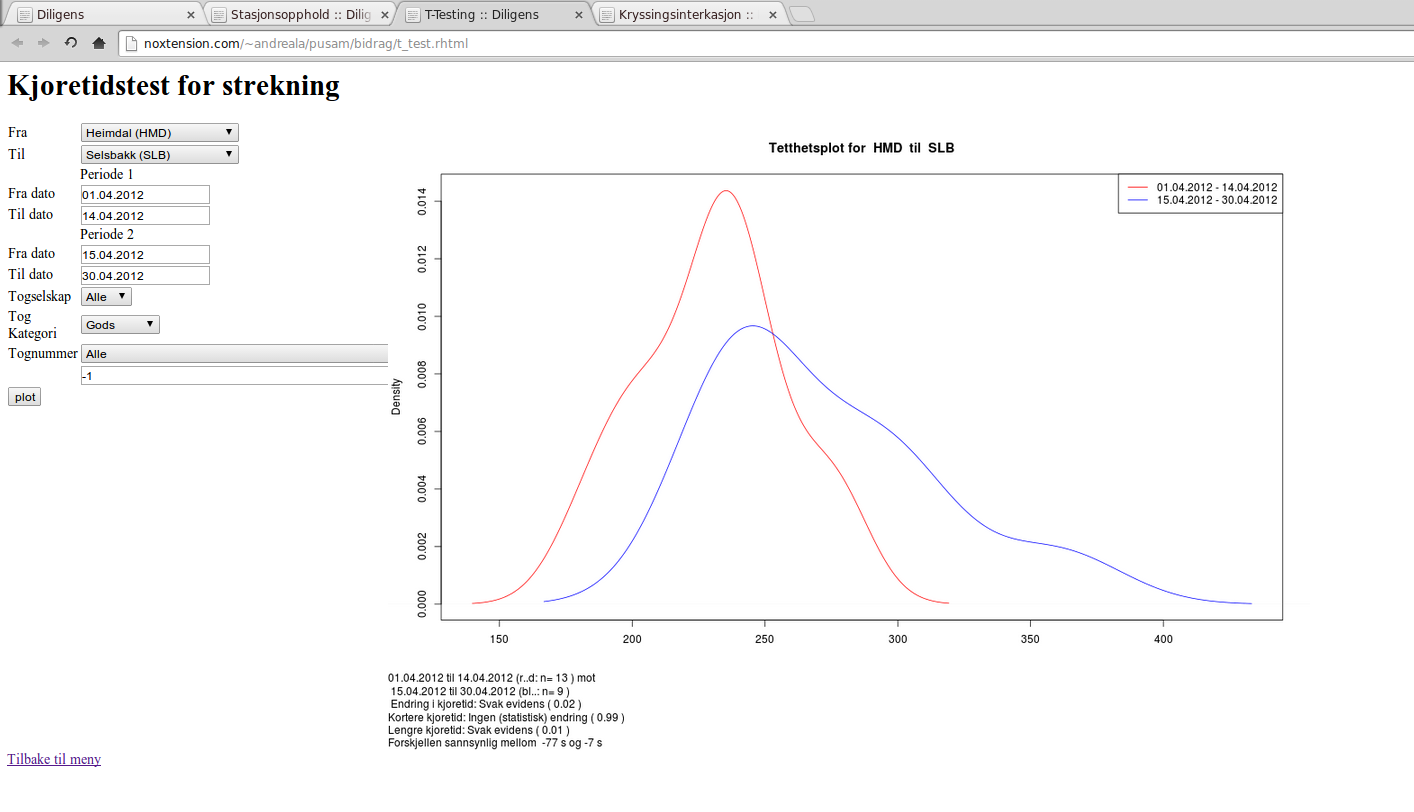
\includegraphics[width=\textwidth,center]{kjoretidstes-strekning.png}
%	\caption[Density plot based on driving time]{Density plot based on driving %time \cite{sintefPresis}}
%	\label{fig:kjoretidstes-strekning}
%\end{figure}
%\pagebreak

\begin{figure}[!htbp]
	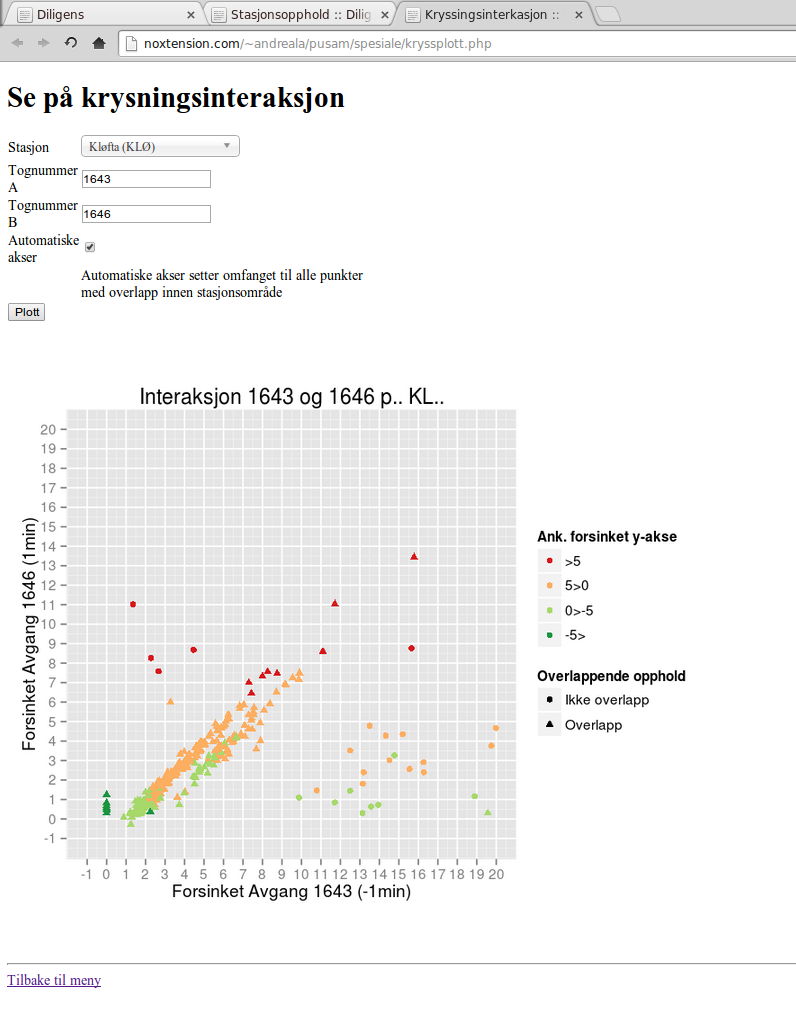
\includegraphics[width=\textwidth,center]{krysningsinteraksjon.png}
	\caption[Train interaction plot]{Train interaction plot \cite{sintefPresis}}
	\label{fig:krysningsinteraksjon}
\end{figure}
\pagebreak

\begin{figure}[!htbp]
	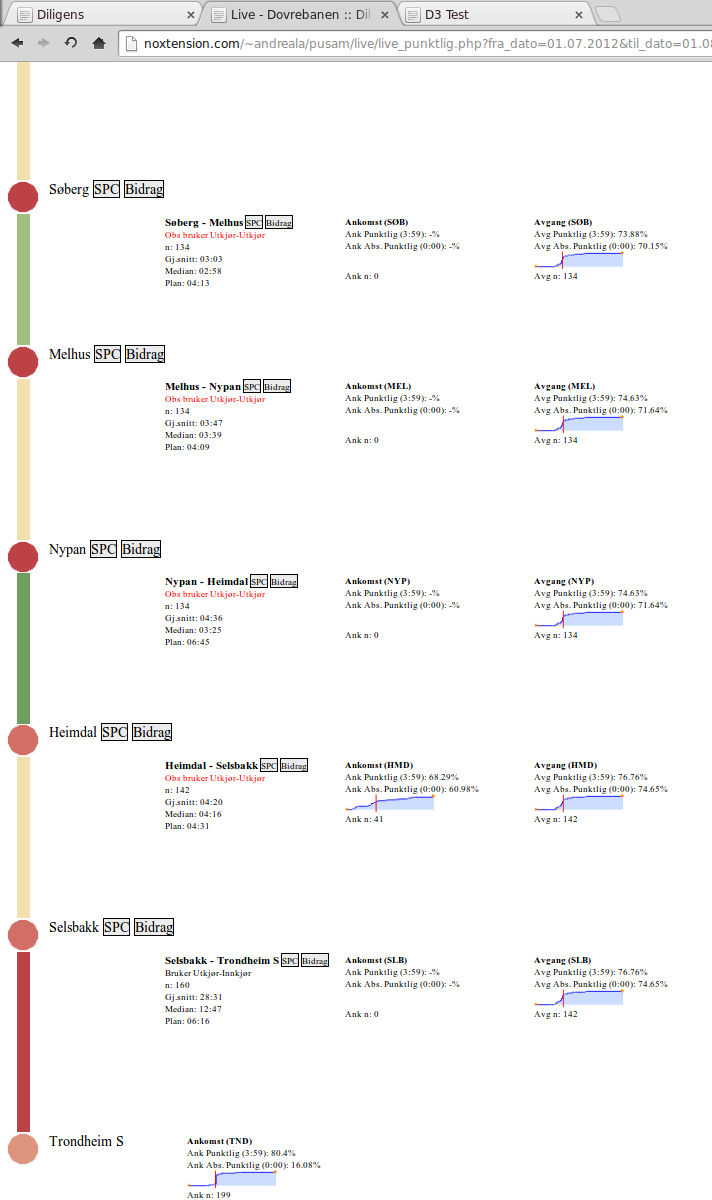
\includegraphics[height=\textheight,center]{live-punklighet.png}
	\caption[Route punctuality]{Route punctuality\cite{sintefPresis}}
	\label{fig:live-punklighet}
\end{figure}
\pagebreak

\begin{figure}[!htbp]
	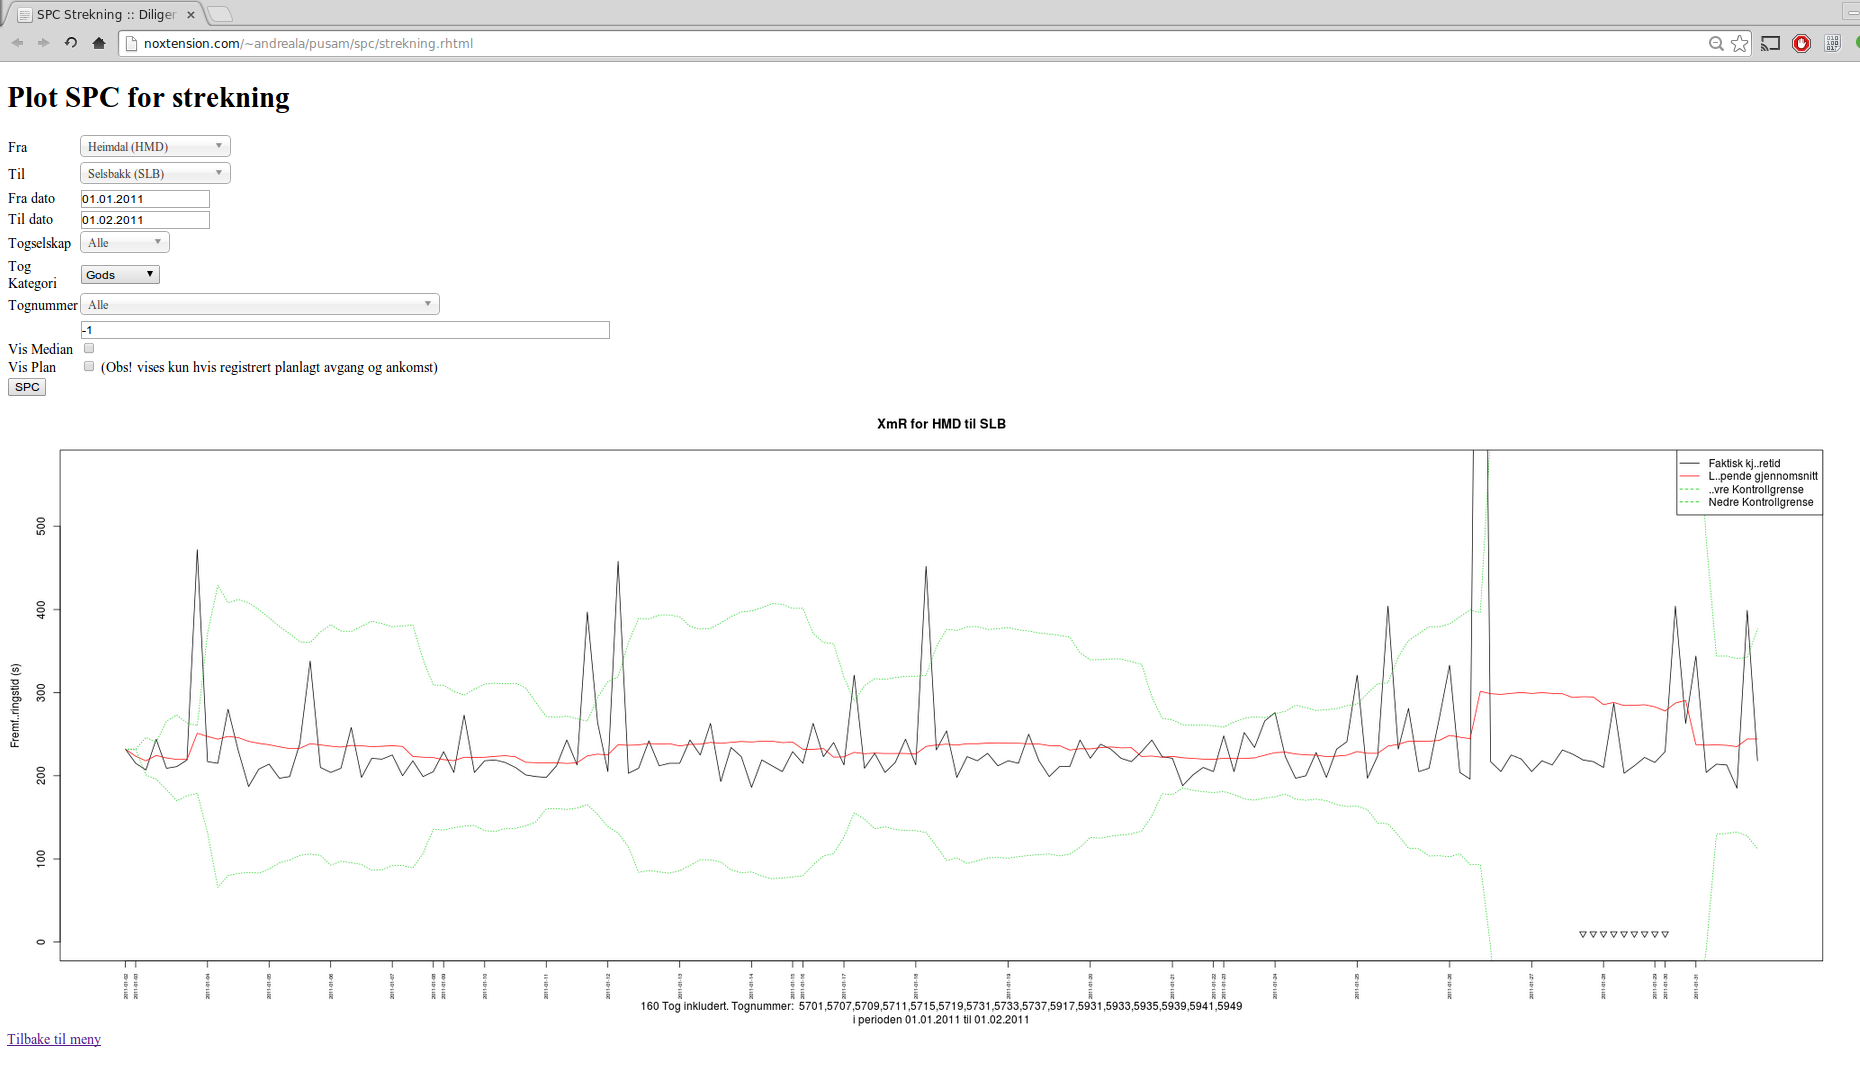
\includegraphics[width=\textwidth,center]{plot-spc-for-strekning.png}
	\caption[SPC Stretch]{SPC Stretch \cite{sintefPresis}}
	\label{fig:plot-spc-for-strekning}
\end{figure}
\pagebreak

\begin{figure}[!htbp]
	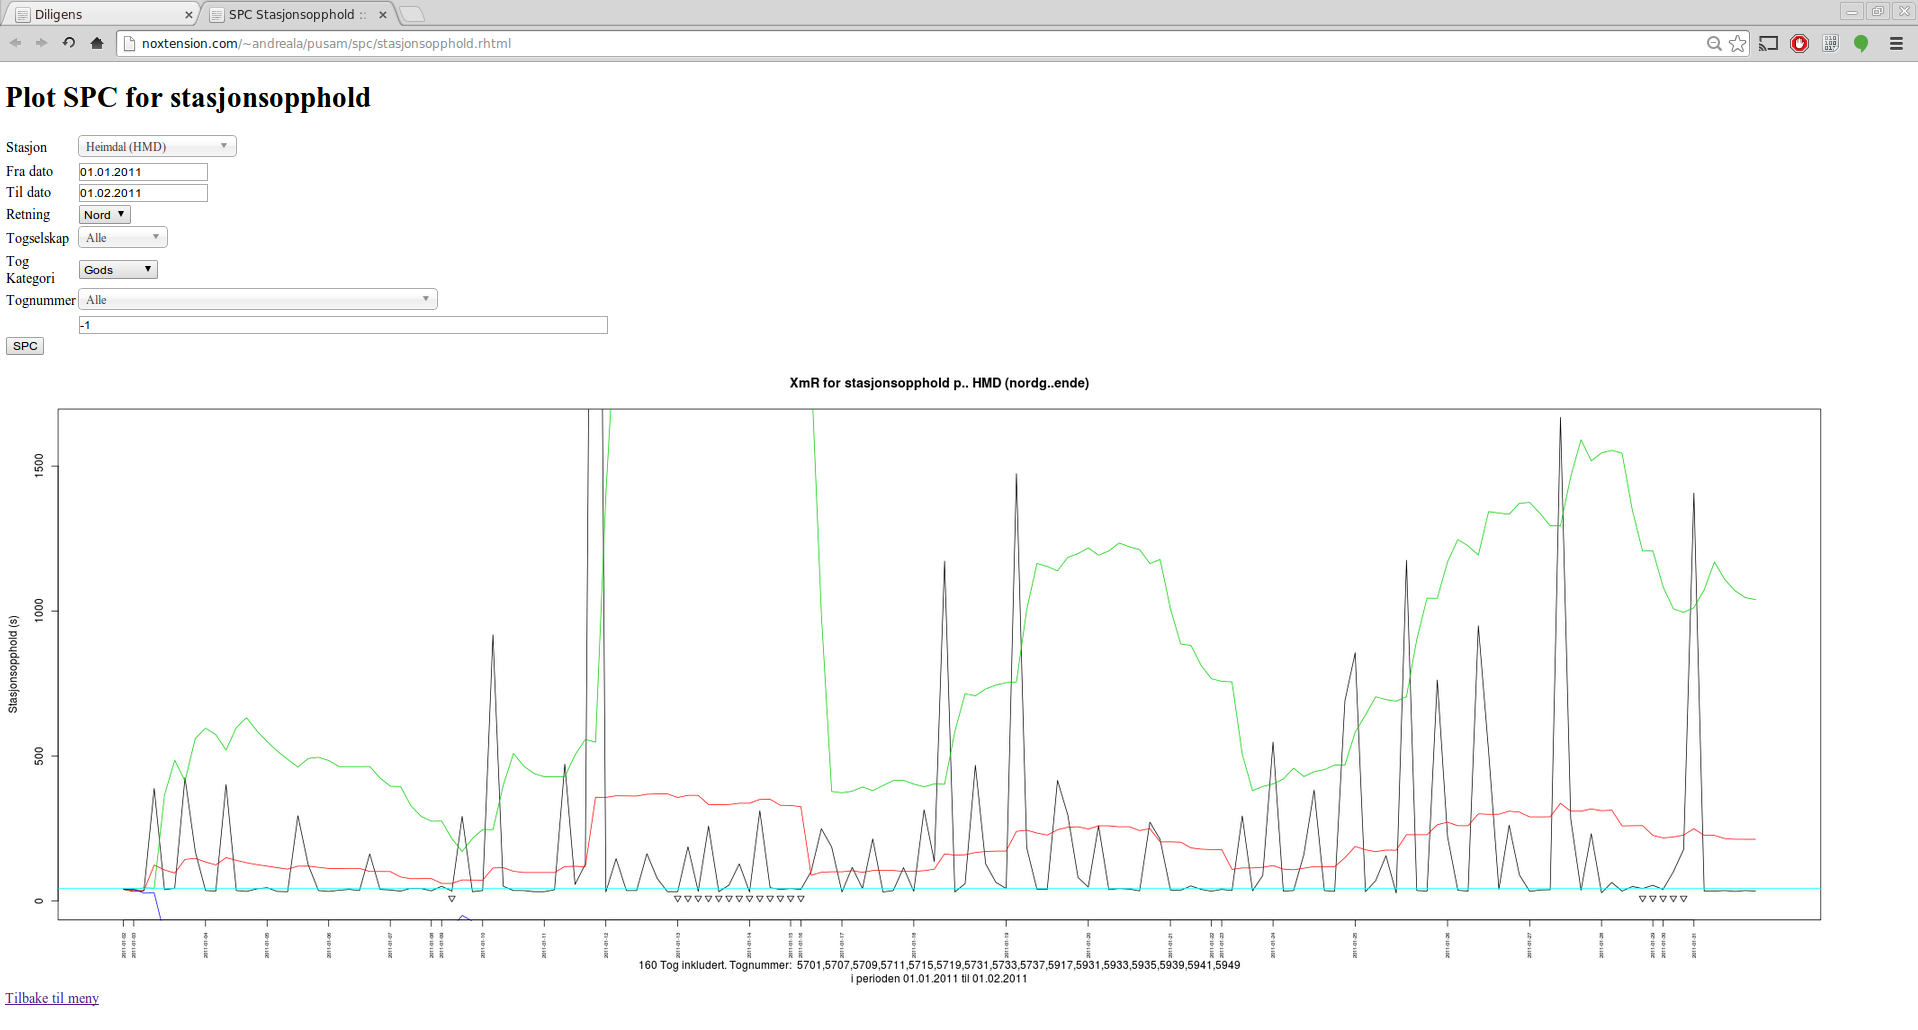
\includegraphics[width=\textwidth,center]{plot-spc-stasjonsopphold.png}
	\caption[SPC Station]{SPC Station \cite{sintefPresis}}
	\label{fig:plot-spc-for-stasjonsopphold}
\end{figure}
\pagebreak

\begin{figure}[!htbp]
	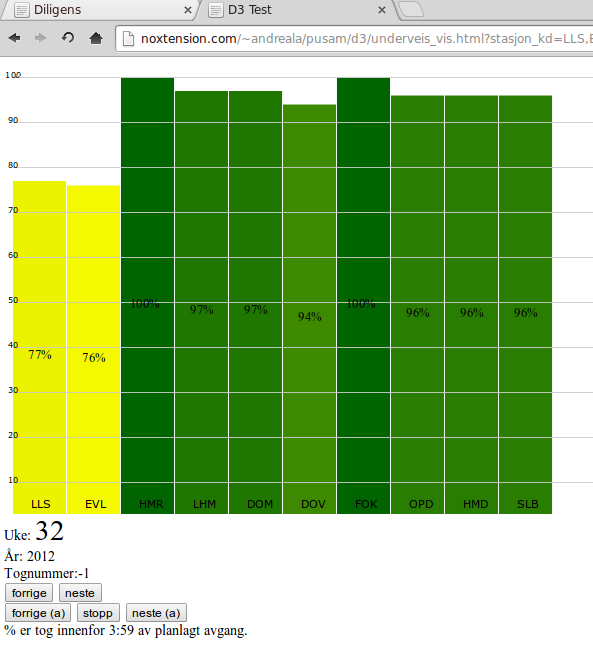
\includegraphics[width=\textwidth,center]{ukespunklighet.png}
	\caption[Weekly punctuality]{Weekly punctuality\cite{sintefPresis}}
	\label{fig:ukespunklighet}
\end{figure}
\pagebreak

\clearpage
\subsection{Cargonet} % (fold)
\label{sub:subsection_cargonet}

% subsection subsection_sintefPresis (end)
Cargonet is a Norwegian which provides intermodal transport on rails. To 
provide a effective tracking service for the customers, Cargonet provides a 
internal service for the users which tracks all trains belonging to Cargonet.
As can be seen in \vref{fig:cargonet}, it only shows a picture of the current
status of each train, it lacks the possibility to analyze every stretch 
individually  and analyze trains and stretches in time.

\begin{figure}[!htbp]
	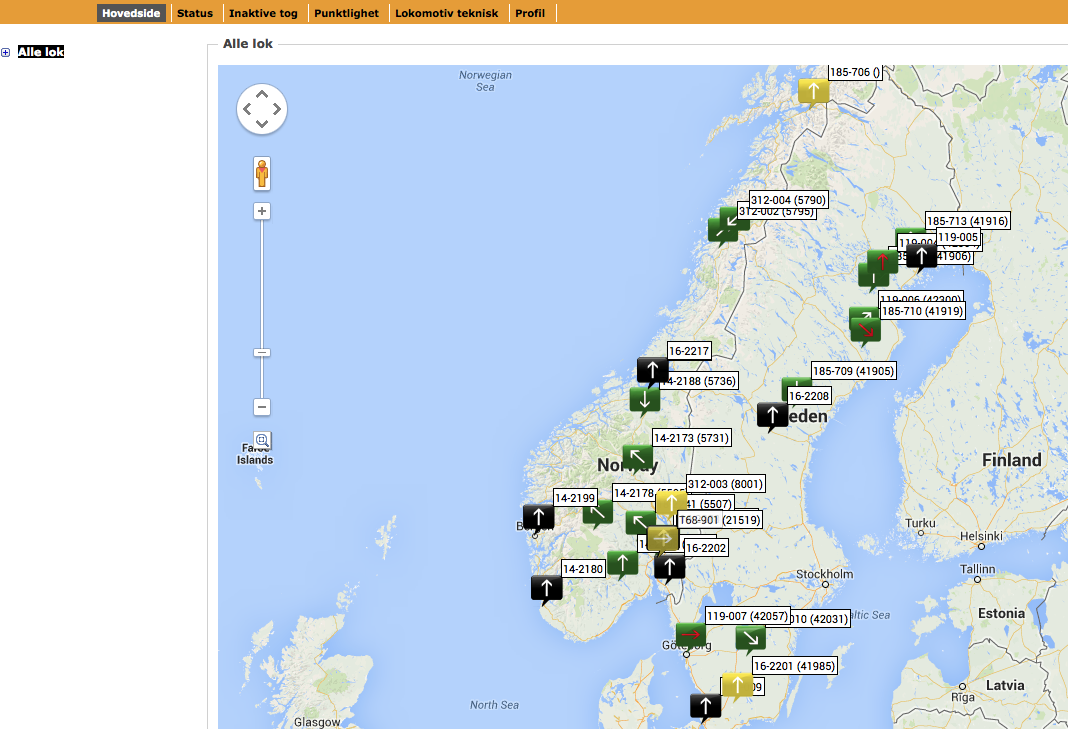
\includegraphics[width=\textwidth,center]{cargonet.png}
	\caption[Cargonet]{Cargonet \cite{cargonet}}
	\label{fig:cargonet}
\end{figure}

\begin{itemize}
	\item [] \textbf{How to read \ref{fig:cargonet}}
	\item Red arrow:\hspace{4ex} Delayed.
	\item White arrow:\hspace{4ex} On time.
	\item Red box:\hspace{4ex} Locomotive driven 2km without carriages.
	\item Black box:\hspace{4ex} Locomotive without carriages.
	\item Yellow box:\hspace{4ex} Locomotive on time without schedule, or known position.
\end{itemize}

\pagebreak
% subsection subsection_cargonet (end)
